\documentclass{standalone}
\usepackage{tikz}
\usepackage{pgfplots}
\pgfplotsset{compat=newest}
\usetikzlibrary{calc}
\usepackage{ifthen}
\newcommand\mycolor{white}
\usetikzlibrary{matrix}

\newcommand\txbox[2]{
    \def\x{3}
    \def\y{2.5}
    \def\h{0.5}
    \def\A{{#1}}
    \node[anchor=north west] (B) at (\A) {R1};
    \node[anchor=south west] (C) at ($(\A) + (0,-2*\h)$) {R2};
    \node (T) at ($(\A) + (8.75*\h,0.5*\h)$) {Output{#2}};
    \node (I) at ($(\A) + (-2.3*\h,-0.6*\h)$) {Input{#2}};
    \foreach \i in {1,...,15}
    {
        \draw ($(\A) + ({(\i+1)*\h},0)$) 
                    rectangle 
                    ($(\A) + ({(\i+2)*\h},-\h)$);
    }
    \node[anchor=south west] (D) at ($(\A) + (1.9*\h,-2.1*\h)$) {$(R2==self.R2)
    \wedge( R1== Rule110(self.R1) )$};
    \draw ($(\A) + (0,-\h)$) -- ($(\A) + (\x,{-\h})$);
    \draw ($(\A) + (2*\h,0)$) -- ($(\A) + (2*\h,-2*\h)$);
    \draw ($(\A)$) rectangle ($(\A) + (17*\h,-2*\h)$);
    \draw ($(\A) + (-0.2*\h, \h)$) rectangle ($(\A) + (17.2*\h,-2.2*\h)$);
    \draw ($(\A) + (-4*\h, 2.5*\h)$) rectangle ($(\A) + (17.4*\h,-2.4*\h)$);
    \draw ($(\A) + (-3.8*\h, \h)$) rectangle ($(\A) + (-0.8*\h,-2.2*\h)$);
    \draw ($(\A) + (-4*\h, 1.5*\h)$) -- node[above, midway] {Transaction {#2}} ($(\A) + (17.4*\h,1.5*\h)$);
    \draw[color=blue,densely dotted, very thick] ($(\A) + (-0.8*\h, -0.6*\h)$) -- ($(\A) + (-0.2*\h,-0.6*\h)$);
}

\begin{document}
    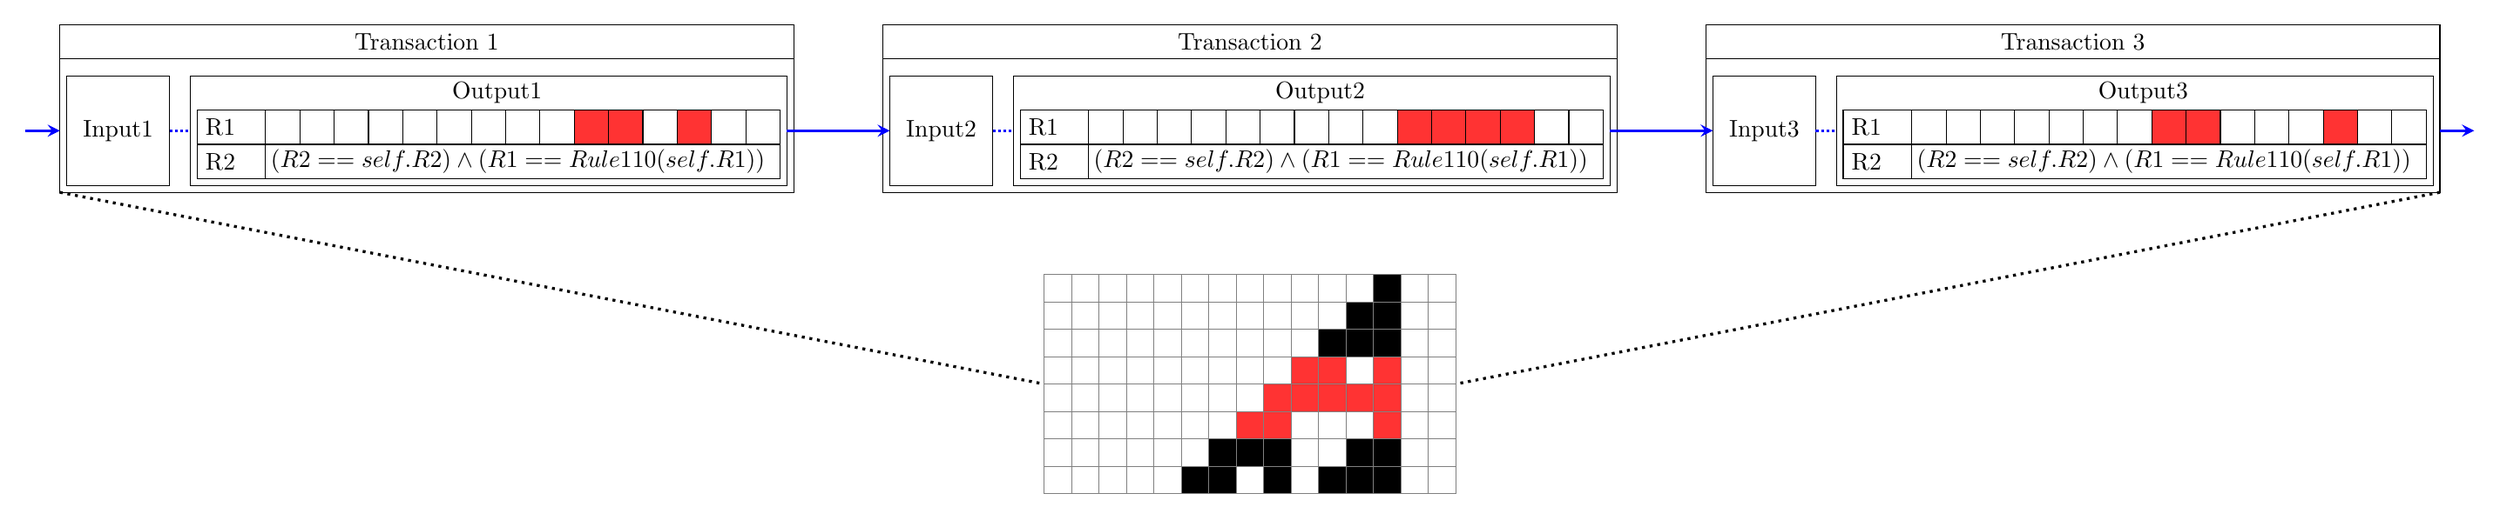
\begin{tikzpicture}[
        X/.style={draw=gray, minimum size=4mm, outer sep=0pt},
        B/.style={X, fill},
        C/.style={X, fill=red!80},
        mymatrix/.style={matrix of nodes, row
            sep=-\pgflinewidth,
            column sep=-\pgflinewidth, nodes={X}, nodes in
        empty cells}
    ]
    \def\h{0.5}
    \txbox{0,0}{1}
    \txbox{12,0}{2}
    \txbox{24,0}{3}
    \draw[->, >=stealth, very thick, blue](-2.5,-0.3) -- (-2,-0.3);
    \draw[->, >=stealth, very thick, blue](8.6,-0.3) -- (10.1,-0.3);
    \draw[->, >=stealth, very thick, blue](20.6,-0.3) -- (22.1,-0.3);
    \draw[->, >=stealth, very thick, blue](32.7,-0.3) -- (33.2,-0.3);
    \draw[very thick, dotted](-2,-1.2) -- (12.35,-4);
    \draw[very thick, dotted](32.7,-1.2) -- (18.35,-4);

    \foreach \i in {5.5,6,7, 17.5,18,18.5,19, 28.5,29, 31}
    {
        \draw[fill=red!80] ($(\i,0)$) rectangle ($({\i+\h},-\h)$);
    }

    \matrix at (15.35,-4) [mymatrix]{
        &&&&&&&&&&&&|[B]|&&\\
        &&&&&&&&&&&|[B]|&|[B]|&&\\
        &&&&&&&&&&|[B]|&|[B]|&|[B]|&&\\
        &&&&&&&&&|[C]|&|[C]|&&|[C]|&&\\
        &&&&&&&&|[C]|&|[C]|&|[C]|&|[C]|&|[C]|&&\\
        &&&&&&&|[C]|&|[C]|&&&&|[C]|&&\\
        &&&&&&|[B]|&|[B]|&|[B]|&&&|[B]|&|[B]|&&\\
        &&&&&|[B]|&|[B]|&&|[B]|&&|[B]|&|[B]|&|[B]|&&\\
    };
    \end{tikzpicture}
\end{document}
